\item \subquestionpointscoding{6} Now add a regularization term to your cross entropy loss.
The loss function will become \begin{equation*}
  J_{MB} = \left(\frac{1}{B}\sum_{i=1}^{B}CE(y^{(i)}, \hat{y}^{(i)})\right) + \lambda \left(||W^{[1]}||^2 + ||W^{[2]}||^2 \right)
  \end{equation*}

Be careful not to regularize the bias/intercept term.
Set $\lambda$ to be 0.0001. Implement the regularized version and plot the same
figures as part (a). Be careful NOT to include the regularization term to measure
the loss value for plotting (i.e., regularization should only be used for gradient calculation for
the purpose of training).

As in the previous part, save the learnt parameters (weights and biases) into a
different file so that we can initialize from them next time.

\clearpage\newpage
If you recreate the plots frmo the previous part, they should look similar to the following:

\begin{figure}[H]
    \centering
    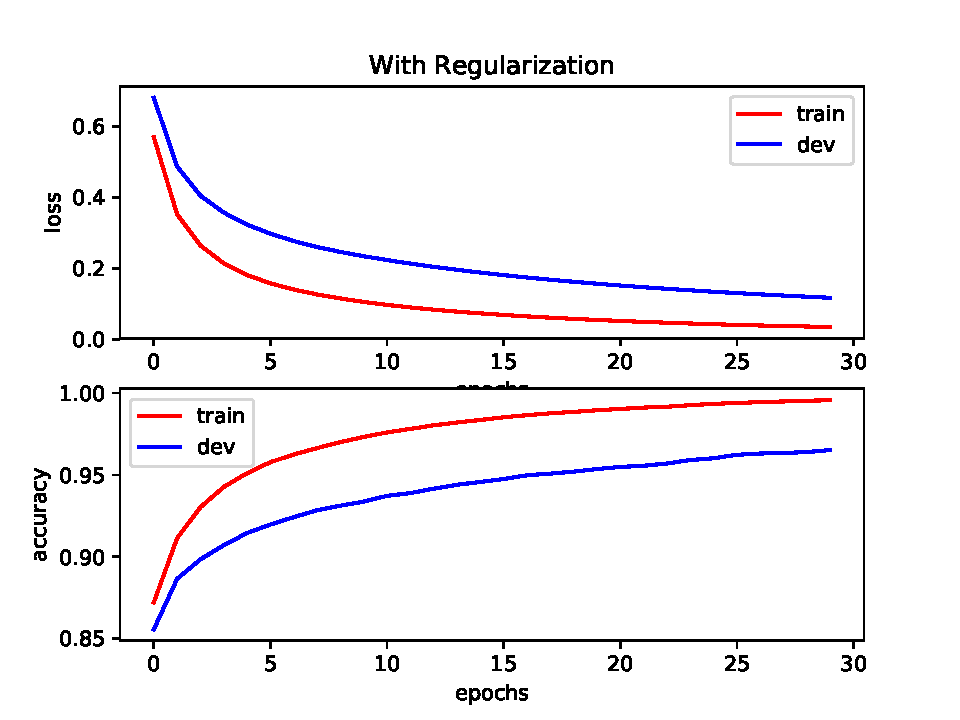
\includegraphics[scale=0.75]{mnist/regularized.pdf}
\end{figure}